%\section{System Analysis And Invariant Formation}
%\label{sec:invariants}
%
%\subsection{Physical System Analysis}
%The physical system must satisfy one out of several criteria in order to be
%stable. The criteria are derived from an analysis of the continuous-time
%dynamics of the system, which are modeled as
%\begin{eqnarray}
%  \frac{d\omega}{dt} &=& -\frac{V_1 V_2}{J \omega X}sin(\theta - \theta_0)-\frac{D}{J}(\omega - \omega_0) + \frac{P_{imb}}{J\omega} - \frac{kP^2}{J\omega}, \nonumber \\
%  \frac{d\theta}{dt} &=& \omega - \omega_0,
%  \label{eqn:swing1}
%\end{eqnarray}
%where $\omega$ is the frequency, $\theta$ is the phase angle of the generator voltage, $\omega_0$ and $\theta_0$ are their nominal
%values, $P_{imb}$ is the net power imbalance due to outstanding messages,
%and the other terms are various physical parameters.  The error energy, given by
%\begin{equation}
%  V(\omega, \theta) = \frac{J}{2} (\omega - \omega_0)^2 + \frac{V_1 V_2}{\omega X}(1-cos(\theta - \theta_0)).
%  \label{eqn:lyap}
%\end{equation}
%is a Lyapunov function (that is, a positive-definite function with a
%non-positive time derivative) if the system satisfies $I_{P1}$, given by
%\begin{equation}
%\left\{
%\begin{matrix}
%I_{P1}: (\omega - \omega_0)^2 \left(D\omega + m \right) \\ + (\omega - \omega_0)(kP^2)  > \delta K (\omega - \omega_0)
%\end{matrix}
%\right\}
%\label{eqn:grid4}
%\end{equation}
%With other factors, $I_{P1}$ ultimately imposes a limit on $\delta * K$, where
%$\delta$ is the quantum of power migrated with each message and $K$ is the
%number of outstanding messages.
%
%In general, if a Lyapunov function exists for a particular physical system, then
%the system is stable. However, there are other conditions that also ensure
%stability for a switched system, which is a continuous-time system that is
%subject to external switching events. A \emph{Lyapunov-like} function
%\cite{branicky98,ye98impulse,ye98hybrid} is similar to a Lyapunov function in
%that it must be positive-definite, but its value may increase under some
%conditions. If the value of the Lyapunov-like function decreases at each
%switching event, then the system is stable. A final option is that the error may
%not decay to zero, but is bounded.
%
%{\bf Physical System Invariant($I_P$).}
%Combining the three conditions, a single invariant may be found,
%\begin{equation}
%  \{I_P : I_{P1} \lor (V(\omega, \theta) < V_{bound}) \lor (V(t) \leq V(t_{x}))\}
%  \label{eqn:IP}
%\end{equation}
%where $V_{bound}$ is the maximum allowable value of $V$, $V(t)$ is the value of
%$V(\omega, \theta)$ at the present time and $V(t_{x})$ is its value at the most
%recent previous violation of $I_{P1}$ due to a large value of $K$. Prior work
%\cite{paul2011,paul12thesis} has demonstrated that the system can be stable for 
%certain combinations of steady-state power imbalance and droop constants in 
%the SST controllers.
 
\section{Adaptive Communication} 
\label{adap_comm}

Physical system stability at any point of time is determined by the product of power migration messages
$K$ in transit and amount of power $\delta$ transferred with every message. 
Stability of network depends only on $K$, where $K$ is a function of rate(s) of power migration
and observed round-trip time between source and receiver nodes in the communication network.
To provide safe and stable operation, an upper bound $Kmax_{global}$ for maximum outstanding messages 
is established prior to power transfer phase, based on physical and network restrictions. $Kmax_{global}$ 
is then distributed as in Figure~\ref{fig:Kmax_distribution} among the nodes that have excess power 
and needs to undergo power migrations. For example, in Equation~\ref{eq:kmax_distrib}, $Kmax_{global}$ 
is distributed among $n$ nodes in proportion to excess power. After distribution, the message scheduling 
algorithm running at node $s$, adapts the power message migration rate $r_s$ or, inversely, the period 
$p_s$ such that the number of outstanding messages of node $s$ at any given time, never exceeds its 
maximum allowed outstanding messages $Kmax_s$.

\begin{equation}
Kmax_s = \lfloor(\frac{P_s}{\sum_{i=1}^{n} P_i}) * Kmax_{global}\rfloor
\label{eq:kmax_distrib}
\end{equation}

\begin{figure}[htb]
  \begin{center}
    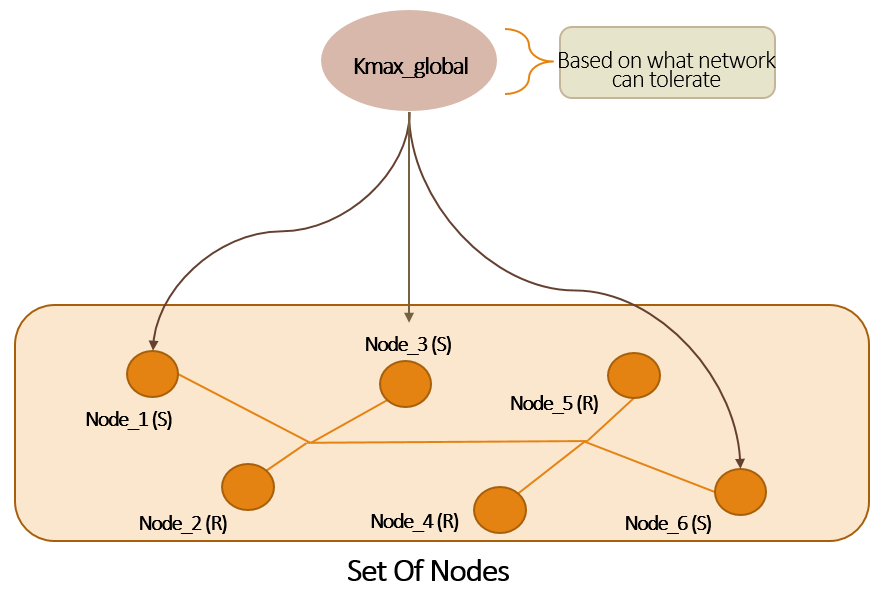
\includegraphics[width=0.45\textwidth]{Figures/kmax_distri.png}
  \caption{$Kmax_{global}$ Distribution Among Sender Nodes}
  \label{fig:Kmax_distribution}
  \end{center}
\end{figure}

\subsection{Scheduling Algorithm}
\label{sec:sched_algo_explanation} 

Every power migrate message initiated by node $s$ is assigned a relative deadline $D_s$ which is determined 
from the current expected response time ($RT_s^{ex}$). Where, $RT_s^{ex}$ is the average of certain number 
of previously observed response times (response time also known as round-trip time). If an acknowledgment 
$m_a$ of message $m$ is not received before its deadline (\textit{deadline miss}) indicates that there 
is a possibility of congestion in the network. Therefore, in an effort to reduce congestion, the algorithm 
increases its expected response time $RT_s^{ex}$ by a pre-defined margin ($RTMargin$) and determines a 
larger transmission period $p_s$ (1/rate) and a larger relative deadline. In the worst case, power migration will only 
be done if acknowledgments for all the outstanding messages are received. Whereas, if certain $CtrMax$ 
(response time counter limit) number of acknowledgments are received consecutively with smaller response 
times than expected, then the algorithm reduces its transmission period (1/$r_s$) and calculates a more tighter 
(smaller) relative deadline, ensuring that physical and network stability is still maintained. Note that 
$RTMargin$ and $CtrMax$ are configurable system parameters and are assumed to be constant for all nodes 
in a given power transfer phase, but in this paper we do make changes to the $CtrMax$ policy in the later 
section. 

Following is a table of events which sets the scheduling algorithm in motion.\\

\begin{scriptsize}
\begin{tabular}{| l | l | l | l |}
	\hline
		&   \textbf{Event Name}	&	\textbf{Sub Event} 			&	\textbf{Function} \\ \hline
	1	&	\textit{Initialize}	&	n/a							&	* Configure and set system parameters \\ \hline
	2	&	\textit{Sent Power}	&	n/a							&	* Assign deadline for message $m$ \\ \hline
	3	&	\textit{Ack Recv}	&	\textit{Better Ack}			&	* Increment $RTCtr$, \\
		&						&								&	IF ($RTCtr=CtrMax$) then \\
		&						&								&	update $r_s, RT_s^{ex}, deadline$ \\
		&						&								&	and reset $RTCtr$. \\
		&						&	\textit{Expected Ack}		&	* Reset $RTCtr$. \\
		&						&	\textit{Ack Of Dln Miss}	&	* IF ($RT_{s(m)}>RT_s^{ex}$) then \\
		&						&								&	update $r_s, RT_s^{ex}, deadline$. \\ \hline	
	4	&	\textit{Dln Miss}	&	n/a							&	* Increment $RT_s^{ex}$ by $RTMargin$ \\
		&						&								&	and update $r_s, RT_s^{ex}, deadline$. \\ \hline
	5	&	\textit{Recv Power}	&	n/a							&	* Send signal to local actuator\\
	\hline
\end{tabular}
\end{scriptsize}


{\bf Message Scheduling Invariant ($I_S$).}

For a given power transfer phase and based on above $Kmax_s$, $p_s$ constraints, following scheduling invariant
$I_s$ can be formed, shown in
Equations \ref{eq:sched_invariant_1} - \ref{eq:sched_invariant_4}.
\begin{equation}
\{I_S = I_k \wedge I_c \wedge I_p\}
\label{eq:sched_invariant_1} 
\end{equation}
\begin{equation}
I_k: K_s < Kmax_s 
\label{eq:sched_invariant_2}
\end{equation}
\begin{equation}
I_c: RT_s^{ex} \leq PT_e - t 
\label{eq:sched_invariant_3}
\end{equation}
\begin{equation}
I_p: t - LT(s) \geq p_s
\label{eq:sched_invariant_4}
\end{equation}

Here, $PT_e$ is the end time of the power transfer phase, $t$ is the time at which
the invariant is evaluated and $LT(s)$ is the time at which the last power
migration message was initiated by node $s$. Work in~\cite{acsmartgrid} shows the necessity of 
conjunction of physical $I_p$ and scheduling $I_s$ invariants in order
to maintain system stability.